\documentclass{aa}
% \documentclass[referee]{aa}
\usepackage[varg]{txfonts}
\usepackage[separate-uncertainty=true]{siunitx}
\usepackage[version=3]{mhchem}
\usepackage[colorlinks, linkcolor=black, citecolor=blue]{hyperref}

\sisetup{range-units = brackets}

\def\eps{\varepsilon}
\def\aap{A\&A}
\def\eprint{e-prints}
\def\apj{ApJ}
\def\apjs{ApJS}
\def\apjl{ApJL}
\def\mnras{MNRAS}
\def\aj{AJ}
\def\nat{Nature}
\def\aaps{A\&A Supp.}
\def\prd{Phys. Rev. D}
\def\prl{Phys. Rev. Lett.}
\def\araa{ARA\&A}

\bibpunct{(}{)}{;}{a}{}{,}


\begin{document}


\title{High resolution near-IR spectroscopy of Arcturus and 10 Leo}
\subtitle{Refining a near-IR iron line list}


\author{ D.~T.~Andreasen\inst{1,2}
    \and S.~G.~Sousa\inst{1}
    \and E.~Delgado Mena\inst{1}
    \and N.~C.~Santos\inst{1,2}
    \and T.~Lebzelter\inst{3}
    \and A.~Mucciarelli\inst{4,5}
    \and J.J.~Neal\inst{1,2}}


\institute{
  Instituto de Astrof\'isica e Ci\^encias do Espa\c{c}o, Universidade do Porto,
  CAUP, Rua das Estrelas, 4150-762 Porto, Portugal,
  \email{daniel.andreasen@astro.up.pt}
\and
  Departamento de F\'isica e Astronomia, Faculdade de Ci\^encias, Universidade
  do Porto, Rua Campo Alegre, 4169-007 Porto, Portugal
\and
  Institute for Astrophysics, University of Vienna, T\"urkenschanzstrasse 17,
  1180 Vienna, Austria
\and
  Dipartimento di Fisica e Astronomia, Universita' degli Studi di Bologna, Viale
  Berti Pichat, 6/2, 40126, Bologna, Italy
\and
  INAF - Osservatorio Astronomico di Bologna, Via Ranzani 1, 40127, Bologna,
  Italy
}





\date{Received ...; accepted ...}

\abstract
% Context
{Reliable stellar atmospheric parameters for FGK stars have been {\bf commonly}
obtained from methods that rely on high resolution and high signal-to-noise
optical spectroscopy. The advent of a new generation of high resolution
{\bf $R>50\,000$} near-IR spectrographs opens the possibility of using classic
spectroscopic methods with high resolution and high signal-to-noise in the NIR
spectral window.}
% Aims
{We aim to obtain precise and accurate atmospheric stellar parameters using high
quality spectra of two K giant stars, Arcturus and 10 Leo.}
% Methods
{Our spectroscopic analysis is based on the iron excitation and ionization
balance done in LTE and a line list of \ion{Fe}{I} and \ion{Fe}{II} lines in the
NIR domain. The line list is being refined from our previous study, allowing us
to obtain more reliable parameters.}
% Results
{{\bf We present a new line list for the derivation of stellar parameters in the
NIR that has allowed us to successfully} obtain parameters for two K giants in
agreement with average literature values adopted.}
% Conclusions
{With these results we are now extending our previous line list towards cooler
stars, thus allowing us to explore the M dwarf stars in the future. {\bf The
improvement of the derivation of stellar parameters for M dwarfs is very
important for the study of the Galactic chemical evolution and crucial for the
characterisation of Earth-like planets, expected to be very common around this
kind of stars.}}



\keywords{data reduction: high resolution spectra --
          stars individual: Arcturus --
          stars individual: 10 Leo}
\maketitle



\section{Introduction}
\label{sec:introduction}

Effective temperature ($T_\mathrm{eff}$), surface gravity ($\log g$),
and metallicity ([M/H], where iron is normally used as a proxy)
are fundamental atmospheric parameters necessary to characterise a single
star, and to indirectly determine other fundamental parameters
such as mass, radius, and age from stellar evolution models
\citep[see e.g.][]{Girardi2000,Dotter2008,Baraffe2015}.
Precise and accurate stellar parameters are also essential in
exoplanet searches. Planetary radius and mass are mainly found from
transit lightcurve analysis and radial velocity analysis, respectively. The
determination of the mass of the planet implies a knowledge of the
stellar mass, while the measurement of the radius of the planet
is dependent on our capability to derive the radius of the star
\citep[see e.g.][]{Torres2008,Ammler2009,Torres2012}.

The derivation of precise stellar atmospheric parameters is not a simple task.
Different approaches often lead to discrepant results
\citep[see e.g.][]{Torres2010,Lebzelter2012b,Santos13}. Interferometry is
usually considered  an accurate method for deriving stellar radii
\citep[see e.g.][]{Boyajian2012}; however, it is only applicable for bright
nearby stars. Asteroseismology, on the other hand, reveals the inner stellar
structure by observing the stellar pulsations at the surface. From
asteroseismology it is possible to measure the surface gravity and mean density,
and therefore to calculate mass and radius with high precision \citep[see
e.g.][]{Kjeldsen1995}. However, for stars on the main sequence asteroseismic
methods can typically only be applied to FG stars, since the oscillation modes
of K and M dwarfs are likely too weak to be detected even with high precision
spectroscopy or photometry. Moreover, the effective temperature is needed when
applying asteroseismology in order to obtain the surface gravity and the mean
density.

A crucial parameter for the indirect determination of stellar bulk properties is
$T_\mathrm{eff}$. In that respect, the infrared flux method (IRFM) has
proven to be reliable for FGK dwarf and subgiant stars. For higher accuracy the
IRFM needs a priori knowledge of the bolometric flux, reddening, surface
gravity, and stellar metallicity
\citep{Blackwell1977,Ramirez2005b,Casagrande2010}.

Finally, the use of high resolution spectroscopy along with stellar atmospheric
models is an extensively tested method that allows the derivation of the
fundamental parameters of a star
\citep[see e.g.][]{Valenti2005,Santos13,Worley2016}. {\bf The procedure depends
on the quality of the spectra, their resolution, wavelength region, and the set
of software used. The latter includes the atmosphere models, radiative transfer
code, and atomic data used.} A fit to the overall spectrum can be applied for
all spectral resolutions, but is often time consuming
\citep[see e.g.][]{Recio2006,Tsantaki2014}. For resolutions larger than
$\lambda/\Delta\lambda > 20\,000$ we can apply the equivalent width (EW) method
\citep[see e.g.][for details]{Tsantaki2013,Andreasen2017a}. However, while the
latter approach is often faster than the synthetic fitting, it requires high
quality spectra, and the star to be a slow rotator (below $\SI{10}{km/s}$ to
$\SI{15}{km/s}$). {\bf It also fails for cool stars due to severe continuum
depression.}

Standard procedures are often used to derive stellar atmospheric parameters from
high quality spectra in the optical \citep[see e.g.][]{Valenti2005,Sousa2008a}.
With the advancement of high resolution near-infrared (NIR) instruments, that is
resolution higher than approximately $50\,000$, we will now be able to use a
similar technique to that used in the optical part of the spectrum
\citep[see e.g.][]{Melendez1999,Sousa2008a,Tsantaki2013,Mucciarelli2013,Bensby2014}.
Such an effort seems very timely because of the growing number of observing
facilities offering a high-resolution access to the near infrared range. At the
moment, the GIANO spectrograph installed at \emph{Telescopio Nazionale Galileo}
(TNG) is already available \citep{GIANO}, as is the \emph{infrared Doppler
instrument} (IRD) installed at the Subaru telescope \citep{IRD}, \emph{Calar
Alto high-Resolution search for M dwarfs with Exoearths with Near-infrared and
optical Échelle Spectrographs} (CARMENES) for the \SI{3.5}{m} telescope at Calar
Alto Observatory \citep{CARMENES}, iShell at the \emph{InfraRed Telescope
Facility} \citep{ishell1,ishell2}. Three new spectrographs are planned for the
near future: 1) The \emph{CRyogenic InfraRed Echelle Spectrograph Upgrade
Project} (CRIRES+) at the \emph{Very Large Telescope} (VLT) \citep{CRIRESp} with
expected first light in 2017, 2) \emph{un SpectroPolarimètre Infra-Rouge A
Near-InfraRed Spectropolarimeter} (SPIRou) at \emph{The Canada-France-Hawaii
Telescope} (CFHT) \citep{SPIROU1,SPIROU2} with expected first light in 2017 as
well, and 3) \emph{Near Infrared Planet Searcher} NIRPS at the ESO 3.6m
telescope in La Silla \citep{NIRPS}. The spectral resolutions for these
spectrographs range between $50\,000$ and $100\,000$.

With the advance of the next generation NIR spectrographs, we are still
preparing the data analysis of stellar spectra, in particular how to get
reliable atmospheric parameters \citep[see e.g.][]{Onehag2012,Lindgren2016,Andreasen2016}.
The analysis of stellar spectra is well understood for FGK stars in the optical
part of the spectrum, however some work still needs to be done for the NIR part.

We continue our series of studies to explore the use of the NIR domain to derive
stellar parameters for FGK and M stars. Here we analyse the atlas of Arcturus
and the spectrum of 10 Leo. For the analysis we use the iron line list presented
in \citet{Andreasen2016} (referred to as Paper I) {\bf which is improved and
update in this work}. In Paper I we successfully tested our method on a slightly
hotter star than the Sun, while in this work we aim to test the method on cooler
stars. The strength of the NIR domain over the optical becomes clear when we
move towards the cooler stars. Here we see less continuum depression and line
blending due to in particular molecular features. Moreover, the cooler stars
emit more light in the NIR domain than the optical, and with the stars with the
lowest masses being intrinsically faint, we thus obtain the majority of the flux
here.



\section{Data}
\label{sec:data}

\subsection{The stars}

While the community is currently on the verge to access large amounts of high
resolution NIR spectra, the available spectra at the moment are sparse. We chose
to use two stars cooler than the Sun since we used a star hotter than the Sun
(HD 20010) in Paper I. {\bf We will however use all four stars in this work for
various reasons. The solar spectrum will be used for inspecting the line list
presented in Paper I. This spectrum was obtained from the Kitt Peak telescope by
\citet{Hinkle1995}. The spectrum of HD 20010 will be reused from Paper I as
well. This spectrum was obtained by the CRIRES spectrograph by
\citet{Lebzelter2012} as part of the CRIRES-POP. HD 20010 will be reanalysed as
to confirm the improvement of the refined line list which will be presented in
the section below. The two stars which we have not analysed before are Arcturus
and 10 Leo. These two extra stars will increase the range of spectral type for
the test of the line list, allowing to test cool giant stars with different
metallicities regimes.}

The atlas of Arcturus (acquired at Kitt Peak National Observatory using the FTS
spectrograph at the Mayall telescope by \citet{Hinkle1995a}), one of the
brightest stars on the Northern hemisphere, covers the spectral range of
interest (YJHK bands). Thus it is well studied \citep[see e.g.][to mention just
a few]{Griffin1967,McWilliam1990,Ramirez2013} {\bf and a benchmark star in
current spectroscopic surveys such as GAIA-ESO \citep{Jofre2014,Smiljanic2014}}.
Strong telluric features were identified with a spectrum from the TAPAS web page
\citep{Bertaux2014}. The atlas also comes with a telluric standard and the ratio
of the two spectra in order to correct for the tellurics. The telluric spectrum
from TAPAS is only used for telluric line identification. We use both the
telluric corrected and non-corrected spectrum.

The spectrum for 10 Leo is {\bf made available by} the CRIRES-POP team
\citep{Nicholls2017}. 10 Leo is very similar to Arcturus, which is also one
reason this star was the first to be fully reduced by the CRIRES-POP team. The
spectrum is divided into several pieces according to the atmospheric windows in
the NIR: YJ (only together), H, K, L, and M. We use only the first three. Some
small gaps are present in the spectrum due to tellurics that could not be
properly removed, low S/N, bad pixels, etc. Rather than giving an uncertain
interpolation, \citet{Nicholls2017} decided to leave small gaps in the data.
This has very little effect on our line by line analysis, however, due to those
gaps, we were unable to measure one \ion{Fe}{II} line which are generally
important to determine the surface gravity.

The data for the two stars are very similar in terms of S/N (around 300 as
measured by IRAF in a continuum region in the YJ band), resolution
(approximately $100\;000$), and spectral coverage. In Fig.~\ref{fig:both} we
compare the spectra of the two stars in a region with some of the iron lines
used for the analysis described below. {\bf The two stars have very similar
spectral type as seen from the two spectra. The difference is shown in the
bottom of the figure in red.}

\begin{figure*}[htpb!]
    \centering
    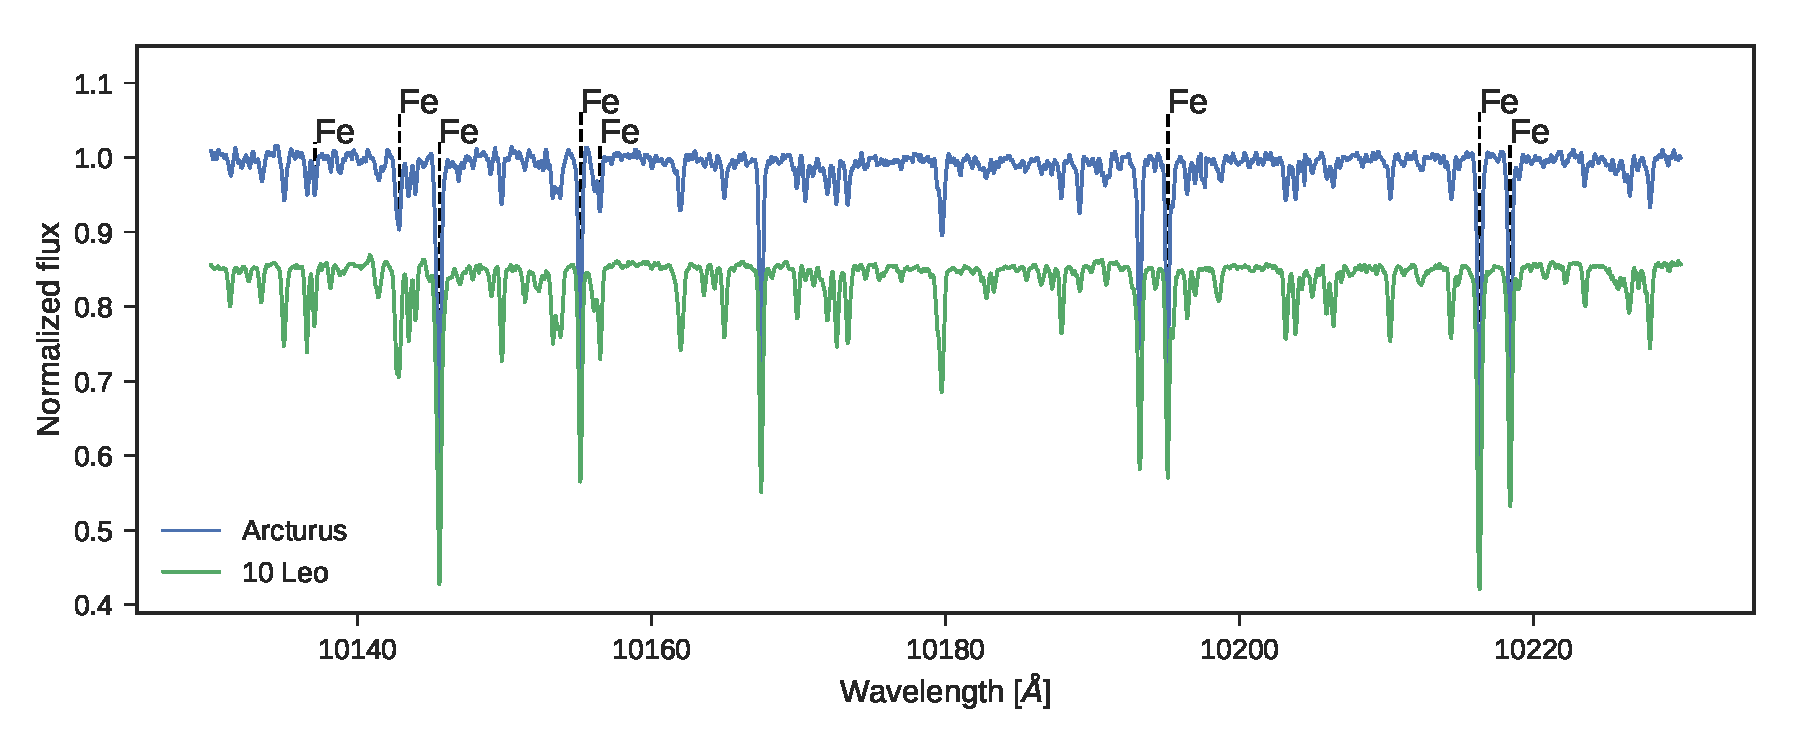
\includegraphics[width=1.0\linewidth]{figures/bothspectra.pdf}
    \caption{Sample spectra of the two stars, Arcturus (blue line), and 10 Leo
             (green line) with an offset. We mark the location of \ion{Fe}{I}
             lines in the region. {\bf The red curve in the bottom represents
             the difference in flux between the two stars, indicating they are
             very similar.}}
    \label{fig:both}
\end{figure*}

A summary of the four stars used can be seen in Table~\ref{tab:stars}. The
parameters are obtained from the PASTEL catalogue \citep{Soubiran2016} which is
a compilation of stellar atmospheric parameters from the literature obtained
mostly from high resolution and high S/N spectra. The parameters are the median
values of all measurements for a given star, where the errors reported are the
standard deviation of this. $\xi_\mathrm{micro}$ is estimated using the
empirical relation by \citet{Tsantaki2013} for dwarf stars, i.e. $\log
g\ge3.95$, and \citet{Adibekyan2015} for the rest. This is done for each
literature value in the catalogue. The value presented in the Table here is
calculated on the same way as the rest of the parameters.
\begin{table*}[htb!]
    \caption{Summary of the four stars used in this work. The stellar parameters
             are from the PASTEL catalogue \citep{Soubiran2016} (see text for
             details), except the parameters for the Sun.}
    \label{tab:stars}
    \centering
    \begin{tabular}{lllllll}
      \hline\hline
        Star        & Spectrographs  & Resolution  & $T_\mathrm{eff}$ (K) &  $\log g$ (dex)  &   $\xi_\mathrm{micro}$ (km/s)   & [Fe/H] (dex)      \\
      \hline
        Sun         & FTS            & 600\,000    & $5777$               &  $4.44$          &    $1.00$                       & $ 0.00$          \\
        Arcturus    & FTS            & 100\,000    & $4300 \pm 111$       &  $1.60 \pm 0.29$ &    $1.93 \pm 0.17$              & $-0.54 \pm 0.11$ \\
        HD 20010    & CRIRES         & 100\,000    & $6152 \pm  95$       &  $3.96 \pm 0.11$ &    $1.17 \pm 0.24$              & $-0.27 \pm 0.06$ \\
        10 Leo      & CRIRES         & 100\,000    & $4742 \pm  61$       &  $2.76 \pm 0.17$ &    $1.45 \pm 0.08$              & $-0.03 \pm 0.02$ \\
      \hline
    \end{tabular}
\end{table*}

\subsection{The line list}

{\bf There have been different recent studies compiling line lists for medium
and high resolution NIR spectra. For M dwarfs there is the line list by
\citet{Onehag2012,Lindgren2016}, which has been tested extensively on CRIRES
spectra ($R\sim100\,000$) using the spectral synthesis method. For FGKM giants
there is the line list used by the APOGEE ($R\sim20\,000$) team compiled by
\citet{Shetrone2015} which only covers the H band.

Since we wanted to compile a line list for FGK, and possible M dwarf stars, we
decided to start from the VALD3 database \citep{VALD1,VALD2}. This has not been
done for the NIR previously.} In Paper I we prepared a \ion{Fe}{I} and
\ion{Fe}{II} line list in the NIR domain. {\bf The atomic data from the lines
were in a wavelength region ranging from \SIrange{10000}{25000}{\AA}, covering
the YJHK bands. EWs were measured for all iron lines with ARES
\citep{Sousa2015a}, discarding any line with EW below \SI{5}{m\AA} or above
\SI{200}{m\AA}. The oscillator strengths of the line list was calibrated using
the solar spectrum, and the solar iron abundance from \citet{Gonzalez2000} at
7.47 dex. The abundances of individual iron lines were obtained with the
radiative transfer code MOOG \citep{Sneden1973} assuming LTE and using ATLAS
model atmospheres \citep{Kurucz1993}.} The line list was successfully used to
derive atmospheric parameters for a late F star, {\bf HD20010}.


\section{Refining the NIR line list}
\label{sec:refining_the_line_list}

{\bf In this work} we will go one step forward, and test {\bf the previous} line
list for {\bf two} K type stars. {\bf Before} testing the line list from Paper I
at cooler effective temperatures with two K stars, it is a primary goal of this
work to refine the line list. This includes identifying recurring outliers (both
from the work done in Paper I and in this work), and lines which we are not able
to measure, e.g. if a line is amidst a forest of telluric lines. {\bf The
refinement is needed, since we experienced some inconsistencies with especially
the derived metallicity compared to literature values. While the metallicity for
HD 20010 (the star analysed in Paper I) were within the errors with those from
the literature, it was over-estimated. The errors on all parameters were also
quite high compared to what is achievable for similar quality spectra from the
visible.} To identify these lines the solar atlas used in Paper I was revisited.
In total 211 out of 295 \ion{Fe}{I} lines and 8 out of 13 \ion{Fe}{II} lines
were removed in the process. Most of these were blended lines with either
tellurics or other stellar lines. This procedure leaves us with 84 \ion{Fe}{I}
lines and 5 \ion{Fe}{II} lines. These lines should be the best for deploying our
technique of determining atmospheric stellar parameters.

During a second look at the Solar spectrum, the EW of the lines were measured by
hand (this had previously been done automatically with ARES). Since we
re-measured the EWs, the oscillator strengths, $\log \mathit{gf}$, had to be
re-calibrated again. Here we simply change the $\log \mathit{gf}$ values for the
measured EW until the abundance of a given line is equal to that of the Sun,
using the same solar atmosphere model as in Paper I. The mean change in $\log
\mathit{gf}$ for common lines is $-0.09 \pm 0.16$. The line list with the
updated $\log \mathit{gf}$ is presented in Appendix~\ref{app:linelist}.

The \ion{Fe}{II} lines are used to determine $\log g$ by imposing ionization
balance with the average \ion{Fe}{I} abundance. However, the low number of
\ion{Fe}{II} lines available is a concern, since the average abundance of
\ion{Fe}{II} is affected more by small number statistics compared to the
numerous \ion{Fe}{I} lines.


\section{Obtaining stellar parameters}
\label{sec:method}

{\bf The method used both in Paper I and here is based on the determination of
the iron abundances on a number of lines from their measured EWs. This is done
using the radiative transfer code MOOG \citep{Sneden1973} to determine the iron
abundance from the measured EWs. Then ionization balance between \ion{Fe}{I} and
\ion{Fe}{II} lines, and excitation balance for all \ion{Fe}{I} lines is imposed,
by changing the atmospheric parameters for the model atmosphere \citep[][ATLAS9
is used here]{Kurucz1993}. While this is a well tested method for getting
atmospheric parameters utilising the optical part of the spectrum, it is a novel
approach in the NIR. Due to its novelty, the measurements of EWs are done with
both manually (IRAF) and automatically (ARES) as a quality check. For both the
automatically and manually measured EWs, we discard all lines with an EW below
$\SI{5}{m}$\AA{} and above $\SI{150}{m}$\AA{} before continuing the analysis. We
decided to be a bit more constrained in the upper limit for the line strength
decreasing it to $\SI{150}{m}$\AA{} to be sure that the Gaussian fit is a good
approximation. Lines outside this range are either too weak to be reliably
measured or saturated and does no longer contain information about the
abundance. The entire procedure of obtaining the stellar parameters is done with
the software FASMA \citep{Andreasen2017a} which does the minimization when
imposing ionization end excitation balance.}




\section{Results}
\label{sec:results}

{\bf The results for the revisited spectrum of HD 20010, and the two additional
K stars are presented here.}

\subsection{Revisiting HD 20010}
\label{sec:hd20010}

As a first step we revisit HD 20010 for which we derived atmospheric stellar
parameters in Paper I using the newly revised line list presented in this paper.
The results are shown in Table \ref{tab:results} along with the {\bf results for
the two other stars analysed in this work}. We see better agreement with the
average literature values adopted (especially $[\ion{Fe}/\ion{H}]$ and $\log g$),
and smaller errors with the updated results. This suggests that the new line
list is more reliable.

\begin{table}[htb!]
    \caption{Results for the three stars with first set of parameters are the
             literature values as presented in Table.~\ref{tab:stars}, second
             set of parameters are results with $\log g$ set to the same value
             during the minimization procedure as found in the literature
             (fixed), and last set of parameters are with all parameters free
             during the minimization procedure.}
    \label{tab:results}
    \centering
    \begin{tabular}{llll}
      \hline\hline
                                    & HD 20010          &  10 Leo           &  Arcturus        \\
      \hline
        Literature                  &                   &                   &                  \\
        $T_\mathrm{eff}$ (lit.)     & $6152 \pm  95$    &  $4741 \pm  60$   & $4300 \pm 110$   \\
        $\log g$ (lit.)             & $3.96 \pm 0.19$   &  $2.76 \pm 0.17$  & $1.60 \pm 0.29$  \\
        $[\ion{Fe}/\ion{H}]$ (lit.) & $-0.27 \pm 0.06$  &  $-0.03 \pm 0.02$ & $-0.54 \pm 0.11$ \\
        $\xi_\mathrm{micro}$ (lit.) & $1.17 \pm 0.24$   &  $1.45 \pm 0.08$  & $1.93 \pm 0.13$  \\
      \hline
        $\log g$ fixed              &                   &                   &                  \\
        $T_\mathrm{eff}$            & $6161 \pm 164$    &  $4761 \pm 118$   & $4357 \pm  74$   \\
        $\log g$                    & 3.96 (fixed)      &  2.76 (fixed)     & 1.60 (fixed)     \\
        $[\ion{Fe}/\ion{H}]$        & $-0.18 \pm 0.11$  &  $ 0.01 \pm 0.07$ & $-0.55 \pm 0.04$ \\
        $\xi_\mathrm{micro}$        & $1.72 \pm 0.44$   &  $1.25 \pm 0.11$  & $1.55 \pm 0.10$  \\
      \hline
        All free                    &                   &                   &                  \\
        $T_\mathrm{eff}$            & $6162 \pm 184$    &  $4805 \pm  98$   & $4439 \pm  62$   \\
        $\log g$                    & $4.08 \pm 0.77$   &  $2.42 \pm 0.61$  & $1.20 \pm 0.20$  \\
        $[\ion{Fe}/\ion{H}]$        & $-0.18 \pm 0.11$  &  $-0.01 \pm 0.07$ & $-0.58 \pm 0.06$ \\
        $\xi_\mathrm{micro}$        & $1.59 \pm 0.49$   &  $1.23 \pm 0.10$  & $1.55 \pm 0.10$  \\
        \hline\hline
    \end{tabular}
\end{table}

{\bf The parameters for the three stars, omitting the Sun since the derived
parameters are trivial with a calibrated line list\footnote{The solar parameters
used were: $T_\mathrm{eff}=\SI{5777}{K}$, $\log g=4.44\,$dex,
$[\ion{Fe}/\ion{H}]=0.00\,$dex, and $\xi_\mathrm{micro}=\SI{1.00}{km/s}$.}, are
presented in Fig.~\ref{fig:parameters}. We show the literature values (blue),
derived parameters with $\log g$ fixed to the literature value (green), and
derived parameters when $\log g$ is free during the minimization procedure (red
points).}

\begin{figure}[htpb!]
    \centering
    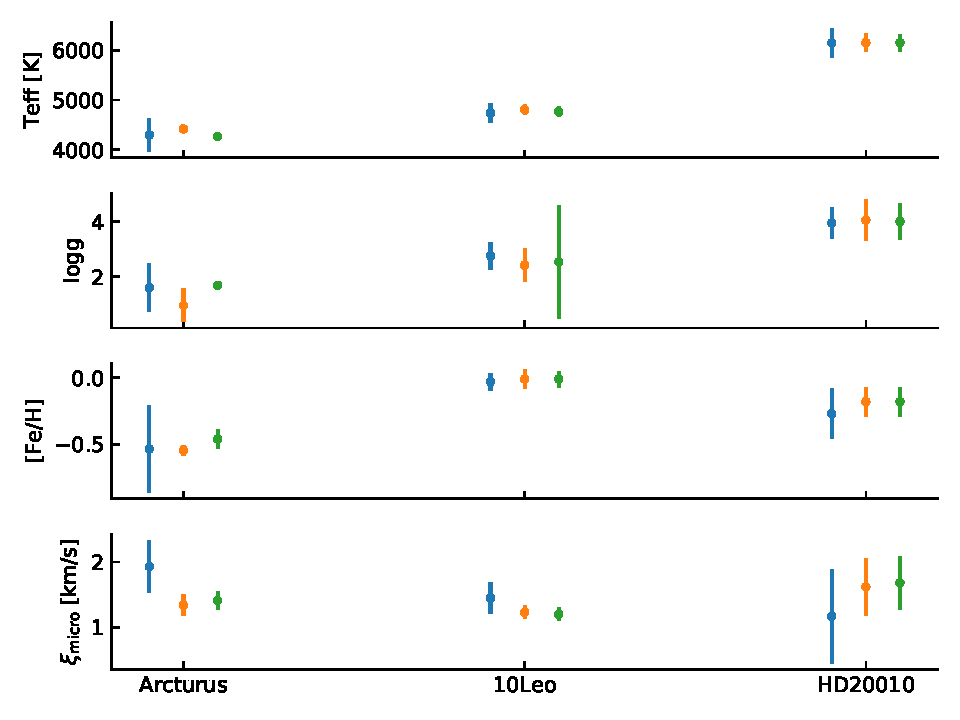
\includegraphics[width=1.0\linewidth]{figures/parameters.pdf}
    \caption{Parameters for Arcturus, 10 Leo, and HD 20010 (revisited in this
             paper). The blue points show the literature values from the PASTEL
             database as discussed in the text. The green points are the
             derived values with $\log g$ fixed to the literature value, and the
             red points show the derived parameters when $\log g$ is also
             derived.}
    \label{fig:parameters}
\end{figure}


\subsection{Arcturus}
\label{sec:arcturus}

Arcturus is one of the brightest stars on the night sky with a V magnitude of
-0.05 \citep{Ducati2002}. Hence it is a prime target for testing with the
numerous measurements of the atmospheric parameters as mentioned above.

The atlas consists of both a summer observation set and a winter observation
set. The two data sets have been obtained in order to minimise the effect of
tellurics at different spectral regions. A comparison between the two sets of
measured EWs - both the manual measurements using IRAF and the automatic
measurements using ARES - are shown in Fig.~\ref{fig:EWcomp}. The automatic EW
measurements for the summer set and winter set show excellent agreement {\bf
with a dispersion of 7m\AA{}}. This means that the two data sets are very
similar, thus we decided to only manually measure the EWs for one set (summer).
We did, however, measure a few lines from the winter data set to verify the
agreement. {\bf Since the EWs are very similar we chose to only derive
parameters of the summer set with EWs measured with ARES.} Parameters were
derived with and without $\log g$ set to a fixed value (1.60\,dex, the average
literature value adopted). The derivation of the parameters followed the
procedure presented in Paper I, although we used the minimization routine from
\citet{Andreasen2017a}. After we reached convergence using all the iron lines we
were able to measure, one outlier above $3\sigma$ in abundance were removed, and
the minimization routine was restarted. This process was done iteratively until
there were no more outliers. The final results are presented in Table
\ref{tab:results} together with mean parameters from the literature.


\begin{figure}[htpb!]
    \centering
    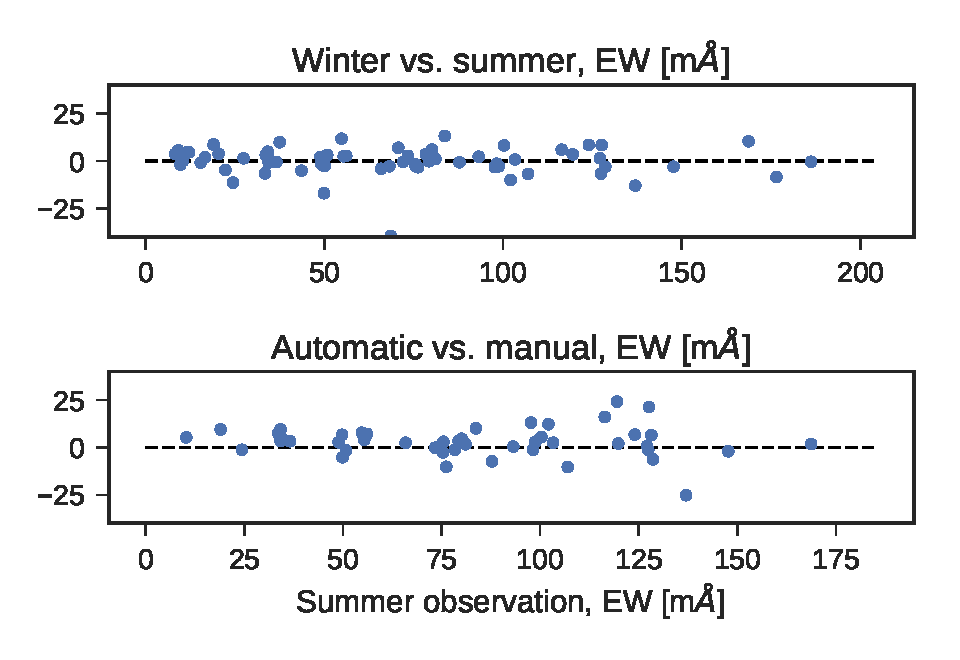
\includegraphics[width=1.0\linewidth]{figures/EWcomp.pdf}
    \caption{Top figure: Difference of the automatic EW measurements between the
             summer observations and winter observations from the Arcturus
             spectra. Bottom figure: Same as above, but with manual measurements
             from ARES (summer) and automatic measurements (summer).}
    \label{fig:EWcomp}
\end{figure}


We generally see good agreement between the derived parameters and the average
values from the literature adopted. The only parameter being difficult to
measure is the surface gravity due to the low number of \ion{Fe}{II} lines in
the NIR. It is very important to derive the metallicity accurately, and we
report consistent results overall, especially with the automatic measurements,
compared to literature values. When measuring the EWs by hand, we might have
systematically overestimated the continuum, resulting in higher
$[\ion{Fe}/\ion{H}]$.


\subsection{10 Leo}
\label{sec:10Leo}

The approach for determining the atmospheric stellar parameters for 10 Leo is
identical to Arcturus. We use ARES on each band (YJ, H, and K-band) separately.
For the small gaps in the spectrum, we simply set the flux to 1, since the
spectrum is already normalised. This will also prevent ARES to identify and
measure any lines in these regions. The EWs from the three regions are combined
to one final line list used for the determination of the parameters. {\bf The
final results can be seen in Fig.~\ref{fig:parameters} and
Table~\ref{tab:results}.}

Generally the derived parameters are in excellent agreement with the literature
values listed here. We were able to derive good $\log g$ values, although with
larger errors compared to the results from the literature. {}



\section{Discussion}
\label{sec:discussion}

\subsection{The role of $\log g$}

One of the most difficult atmospheric stellar parameters to get from a spectrum
is the surface gravity. For this we need the lines of pressure sensitive ionized
atoms such as \ion{Fe}{II}. However, they are more sparse than neutral iron,
\ion{Fe}{I}, making the determination more challenging. This is true in the
optical \citep[see e.g. the discussion by][]{Mortier2013c}, and even more in the
NIR (see e.g. Paper I). One solution to this problem is to fix the value of
surface gravity and derive the other parameters. With the parallaxes from e.g.
Gaia \citep{GAIA} we will have access to accurate $\log g$. However, this
requires a priori knowledge of the mass from e.g. isochrones, and
$T_\mathrm{eff}$. By iteratively obtaining the $T_\mathrm{eff}$ from
spectroscopy and the corresponding $\log g$ from the parallaxes, we can obtain
reliable $T_\mathrm{eff}$, $\log g$, and $[\ion{Fe}/\ion{H}]$. {\bf Another
approach is to use asteroseismic $\log g$ which are becoming a new standard.
This has previously been done in the APOGEE+\emph{Kepler} (APOKASC) context by
\citet{Pinsonneault2014,Hawkins2016}. It is important to mention, that the
asteroseismic $\log g$ in turn is dependent on $T_\mathrm{eff}$ through the
scaling relations \citep[see e.g.][]{Kjeldsen1995}. Moreover, this is not
possible for all spectral classes. It is e.g. not possible for M stars, since no
pulsations have been observed here.}

Since there is a dependence between the other derived parameters with $\log g$,
simply using a mean value as a reference value can lead to misleading
parameters. To verify the impact of using the wrong $\log g$ as baseline, we
tested what was the $T_\mathrm{eff}$ and $[\ion{Fe}/\ion{H}]$ that we derive by
setting $\log g$ fixed to values between 0.9\,dex and 2.2\,dex, i.e., in the
range of the literature values found. The results show that $T_\mathrm{eff}$ and
$[\ion{Fe}/\ion{H}]$ can change by $\SI{200}{K}$ and 0.21\,dex, respectively.
This is most likely the origin of the small discrepancies seen for the
parameters of Arcturus when the $\log g$ is fixed and free.

Note that the ionized iron lines are not only sparse, they are also rather weak.
The lowest measured EW for an \ion{Fe}{II} line is $\SI{7.8}{m}$\AA{} (in
Arcturus), while the highest measured value is $\SI{20.7}{m}$\AA{} (in 10 Leo).
However, with the upcoming high quality spectra for the NIR, the community
should still be able to measure these \ion{Fe}{II} lines. We showed in Paper I
that a minimum S/N of around 50 is required to utilise this method, however this
was only tested for the Sun, and a higher S/N might be needed for other spectral
types.


\subsection{Proper data reduction}

The relative novelty of NIR high resolution spectroscopy is reflected on a
number of problems regarding the available spectra that made our analysis
particularly difficult. For instance, in Paper I we had to deal with a less
reliable wavelength calibration for the spectrum of HD 20010. This meant the
wavelength was stretched when compared to a synthetic spectrum, which is
discussed in more detail by \citet{Nicholls2017}. The poor wavelength
calibration for HD 20010 most likely caused bad EW measurements. In addition,
the spectrum was not corrected for telluric lines which also caused minor
deviation from the true EW when measured. Another reason was the non-refined
line list used, which we have attempted to correct for here. The refined line
list has made the derivation of the metallicity more reliable compared with the
adopted literature as it is demonstrated in Sec.~\ref{sec:hd20010}. It is
expected that even better results will be obtained for this star once the final
spectrum is presented by the CRIRES-POP team.

All the above problems we had with HD 20010 have been solved for 10 Leo, and it
is clear the results are of much higher quality. This can be seen by the smaller
errors we have on our parameters, and the good agreement of all parameters
compared with the literature. Therefore, it may be necessary that a telluric
correction is applied to the spectrum before atmospheric stellar parameters can
be determined reliably. However, with our limited sample it is difficult to make
a clear conclusion yet. Note that this is unlike the optical where a telluric
correction is not necessary for obtaining atmospheric parameters.


\subsection{The refined line list}

{\bf The line list from Paper I has been refined, i.e. several blended or
otherwise unreliable measured lines has been removed. This was done using the
same solar spectrum as in Paper I. In order to test this new line list it was
first used to re-derive parameters for HD 20010, which was the test case in
Paper I. Using the refined line list we were able to reduce the error, and
derive parameters closer to the literature values. Especially important are the
derived metallicity which were previously over-estimated with $\sim0.1$ dex.
With the refined line list the metallicity went from $-0.14\pm0.14$ dex to
$-0.18\pm0.11$, so an overall improvement.

Furthermore, the refined line list was tested on the two K giants, Arcturus and
10 Leo. We see a good agreement between the derived parameters and the
literature values used for comparison.

While this line list, and in particular this method for obtaining stellar
atmospheric parameters, will fail at higher $T_\mathrm{eff}$, above
$\sim\SI{7000}{K}$\footnote{Due to the low number of absorption lines and
non-LTE effects.} it should still work at lower $T_\mathrm{eff}$. The biggest
challenge in this regime is the continuum depression by molecular lines, however
this is a smaller effect compared with the optical part of the spectrum. Hence
it will still be interesting to see how far this line list might work in terms
of $T_\mathrm{eff}$.}



\section{Conclusion}
\label{sec:conclusion}

In this paper we presented a refined \ion{Fe}{I} and \ion{Fe}{II} line list in
the NIR domain {\bf to derive parameters for high resolution spectra}. The
method should work in all spectral ranges, however, it is important to locate
the appropriate iron lines. For the NIR we need a relative large coverage (YJHK,
although few lines are in the K band). The method used here which is usually
adopted in the optical domain to derive parameters is now available for the NIR
as well. The refined line list has been used to derive new parameters for the
late F-star HD 20010, as well as for two K-giants (Arcturus and 10 Leo). The
results show that the stellar atmospheric parameters derived using our line list
are perfectly compatible with the literature values. We are thus now extending
the line list towards cooler temperatures. With the updated results for HD
20010, and the results for Arcturus and 10 Leo, we are now reaching the same
precision that has been reached in the optical for similar spectral types using
the same methodology. The obvious next step is to approach the even cooler M
stars. Particular interesting are the M dwarf stars, known to be prone forming
rocky planets. As important as cooler stars, we have yet to test our line list
on any dwarf stars other than the Sun for which our line list is calibrated. The
upcoming spectral library from CARMENES (priv. comm. with P. Amado) will provide
the community with high quality spectra and allow us to extend our test to many
different spectral types of interest.



\begin{acknowledgements}

We thank Jos\'e Caballero for many useful comments during the process which
led to this paper.

This work was supported by Funda\c{c}\~ao para a Ci\^encia e a Tecnologia, FCT,
(ref. UID/FIS/04434/2013, PTDC/FIS-AST/1526/2014, and PTDC/FIS-AST/7073/2014)
through national funds and by FEDER through COMPETE2020 (ref.
POCI-01-0145-FEDER-007672, POCI-01-0145-FEDER-016886, and
POCI-01-0145-FEDER-016880). N.C.S., and S.G.S. acknowledge the support from FCT
through Investigador FCT contracts of reference IF/00169/2012, and
IF/00028/2014, respectively, and POPH/FSE (EC) by FEDER funding through the
program “Programa Operacional de Factores de Competitividade - COMPETE”. E.D.M
acknowledge the support from the FCT in the form of the grants
IF/00849/2015/CP1273/CT0003. JJN acknowledges support from FCT in the form of a
“PhD::Space” (PD/00040/2012) network doctoral grant, of reference
PD/BD/52700/2014.

This research has made use of the SIMBAD database operated at CDS, Strasbourg
(France).

\end{acknowledgements}


\bibliographystyle{aa}
\bibliography{thesis}

\begin{appendix}

\section{Complete refined line list}
\label{app:linelist}

The complete refined line list with Solar EWs measured by hand using IRAF, {\bf
and the three stars also analysed in this work. Note that the EWs given here are
after removal of outliers in abundance. This is done automatically with FASMA
\citep{Andreasen2017a}.}

\begin{onecolumn}
  \begin{longtable}{cclrrrrr}
      \caption{\label{tab:linelist} Refined line list with all \ion{Fe}{I} and
               \ion{Fe}{II} lines and corresponding atomic data, including the
               updated $\log \mathit{gf}$. The four last columns are the
               measured EWs in m\AA{} for the four stars analysed in this work.
               This table is available in an electronic form online.}\\
        \hline\hline
          Wavelength (\AA) & Element        & EP (eV)  &  $\log \mathit{gf}$  &  Sun  & HD 20010  & 10 Leo & Arcturus \\
        \hline
        \endfirsthead
        \caption{continued.}\\
        \hline\hline
          Wavelength (\AA) & Element        & EP (eV)  &  $\log \mathit{gf}$  &  Sun  & HD 20010  & 10 Leo & Arcturus \\
        \hline
        \endhead
          10065.05         & \ion{Fe}{I}    &  4.83    &    -0.279            &  94.0 &  ...      & 115.2  & 107.0    \\
          10080.42         & \ion{Fe}{I}    &  5.10    &    -1.964            &   5.9 &  ...      &  ...   & ...      \\
          10081.39         & \ion{Fe}{I}    &  2.42    &    -4.512            &   6.9 &  ...      &  42.9  &  49.8    \\
          10086.24         & \ion{Fe}{I}    &  2.95    &    -3.978            &   7.0 &  39.5     &  34.2  & ...      \\
          10137.10         & \ion{Fe}{I}    &  5.09    &    -1.736            &   9.8 &  ...      &  21.1  &  12.1    \\
          10142.84         & \ion{Fe}{I}    &  5.06    &    -1.554            &  14.9 &   5.5     &  36.3  & ...      \\
          10145.56         & \ion{Fe}{I}    &  4.80    &    -0.118            & 109.0 & 146.5     & 137.0  & ...      \\
          10155.16         & \ion{Fe}{I}    &  2.18    &    -4.336            &  16.2 &  79.0     &  87.8  & ...      \\
          10156.51         & \ion{Fe}{I}    &  4.59    &    -2.109            &  12.2 &  ...      &  29.2  &  24.4    \\
          10167.47         & \ion{Fe}{I}    &  2.20    &    -2.319            & 125.7 &  ...      &  ...   & ...      \\
          10195.11         & \ion{Fe}{I}    &  2.73    &    -3.608            &  22.6 &  10.7     &  76.3  &  78.4    \\
          10216.31         & \ion{Fe}{I}    &  4.73    &     0.047            & 129.9 & 144.9     & 128.6  & ...      \\
          10218.41         & \ion{Fe}{I}    &  3.07    &    -2.893            &  40.9 & 101.7     &  98.2  & ...      \\
          10265.22         & \ion{Fe}{I}    &  2.22    &    -4.648            &   8.1 &  ...      &  52.6  &  55.4    \\
          10307.45         & \ion{Fe}{I}    &  4.59    &    -2.432            &   6.4 &  16.8     &   9.1  & ...      \\
          10332.33         & \ion{Fe}{I}    &  3.63    &    -3.131            &  10.5 &  ...      &  48.6  &  34.4    \\
          10340.89         & \ion{Fe}{I}    &  2.20    &    -3.665            &  46.6 & 116.5     & 127.1  & ...      \\
          10347.97         & \ion{Fe}{I}    &  5.39    &    -0.717            &  37.0 &  19.5     &  58.2  &  36.6    \\
          10353.81         & \ion{Fe}{I}    &  5.39    &    -0.989            &  24.2 &  12.1     &  39.6  &  33.4    \\
          10364.06         & \ion{Fe}{I}    &  5.45    &    -1.100            &  18.0 &   9.0     &  33.5  &  16.6    \\
          10379.00         & \ion{Fe}{I}    &  2.22    &    -4.236            &  18.7 &   6.2     &  76.4  &  80.1    \\
          10388.75         & \ion{Fe}{I}    &  5.45    &    -1.471            &   8.7 &  ...      &  16.5  &   8.2    \\
          10395.80         & \ion{Fe}{I}    &  2.18    &    -3.435            &  61.3 & 129.3     & 147.7  & ...      \\
          10423.03         & \ion{Fe}{I}    &  2.69    &    -3.658            &  22.9 &   8.4     &  80.6  &  79.3    \\
          10423.74         & \ion{Fe}{I}    &  3.07    &    -3.119            &  29.9 &  ...      &  ...   & ...      \\
          10469.65         & \ion{Fe}{I}    &  3.88    &    -1.277            &  89.3 & 131.9     & 127.4  & ...      \\
          10532.24         & \ion{Fe}{I}    &  3.93    &    -1.650            &  64.4 & 109.1     &  98.8  & ...      \\
          10555.65         & \ion{Fe}{I}    &  5.45    &    -1.282            &  13.1 &   7.1     &  25.5  &  15.4    \\
          10577.14         & \ion{Fe}{I}    &  3.30    &    -3.222            &  17.2 &   6.0     &  67.0  &  56.1    \\
          10616.72         & \ion{Fe}{I}    &  3.27    &    -3.306            &  15.6 &   6.5     &  57.0  &  50.8    \\
          10725.19         & \ion{Fe}{I}    &  3.64    &    -2.948            &  15.7 &   6.8     &  57.5  &  48.9    \\
          10753.00         & \ion{Fe}{I}    &  3.96    &    -2.077            &  39.7 &  81.8     &  73.4  & ...      \\
          10780.69         & \ion{Fe}{I}    &  3.24    &    -3.553            &  10.4 &  ...      &  49.7  &  34.2    \\
          10783.05         & \ion{Fe}{I}    &  3.11    &    -2.786            &  47.0 & 100.4     & 103.3  & ...      \\
          10818.28         & \ion{Fe}{I}    &  3.96    &    -2.160            &  35.6 &  20.3     &  76.2  & ...      \\
          10863.52         & \ion{Fe}{I}    &  4.73    &    -0.877            &  67.1 &  84.2     &  75.4  & ...      \\
          10884.26         & \ion{Fe}{I}    &  3.93    &    -2.129            &  39.1 &  79.3     &  75.5  & ...      \\
          10896.30         & \ion{Fe}{I}    &  3.07    &    -2.911            &  42.9 & 101.8     & 100.3  & ...      \\
          11013.24         & \ion{Fe}{I}    &  4.80    &    -1.240            &  42.4 &  ...      &  ...   & ...      \\
          11026.79         & \ion{Fe}{I}    &  3.94    &    -2.517            &  21.2 &  49.4     &  68.6  & ...      \\
          11119.80         & \ion{Fe}{I}    &  2.85    &    -2.452            &  84.8 & 142.5     &  ...   & ...      \\
          11641.80         & \ion{Fe}{I}    &  4.58    &    -2.116            &  15.6 &  ...      &  ...   & ...      \\
          11778.42         & \ion{Fe}{I}    &  5.34    &    -1.708            &   8.4 &  6.3      &  11.2  & ...      \\
          12053.08         & \ion{Fe}{I}    &  4.56    &    -1.602            &  41.3 &  33.5     &  76.5  & ...      \\
          12119.50         & \ion{Fe}{I}    &  4.59    &    -1.897            &  25.0 &  ...      &  50.1  & ...      \\
          12213.34         & \ion{Fe}{I}    &  4.64    &    -2.006            &  19.1 &  16.5     &  37.5  & ...      \\
          12227.11         & \ion{Fe}{I}    &  4.61    &    -1.408            &  51.5 &  ...      &  72.0  & ...      \\
          12244.92         & \ion{Fe}{I}    &  3.64    &    -3.222            &  11.8 &  54.2     &  ...   & ...      \\
          12340.48         & \ion{Fe}{I}    &  2.28    &    -4.680            &   9.4 &  ...      &  58.2  &  54.8    \\
          12342.92         & \ion{Fe}{I}    &  4.64    &    -1.545            &  42.1 &  19.4     &  80.4  &  65.9    \\
          12510.52         & \ion{Fe}{I}    &  4.96    &    -1.930            &  12.9 &  39.1     &  20.4  & ...      \\
          12557.00         & \ion{Fe}{I}    &  2.28    &    -4.026            &  33.8 &  14.6     & 113.7  & 124.0    \\
          12615.93         & \ion{Fe}{I}    &  4.64    &    -1.686            &  35.7 &  ...      &  44.1  & ...      \\
          12638.70         & \ion{Fe}{I}    &  4.56    &    -0.679            & 112.3 &  ...      &  ...   & ...      \\
          12807.15         & \ion{Fe}{I}    &  3.64    &    -2.649            &  37.1 &  ...      &  97.7  & ...      \\
          12808.24         & \ion{Fe}{I}    &  4.99    &    -1.811            &  16.4 &   9.8     &  47.9  &  33.6    \\
          12824.86         & \ion{Fe}{I}    &  3.02    &    -3.612            &  20.1 &   6.6     &  84.1  &  83.7    \\
          12840.57         & \ion{Fe}{I}    &  4.96    &    -1.612            &  25.3 &  10.9     &  72.1  & ...      \\
          12879.77         & \ion{Fe}{I}    &  2.28    &    -3.525            &  68.7 & 126.2     & 168.7  & ...      \\
          12896.12         & \ion{Fe}{I}    &  4.91    &    -1.713            &  23.2 &  12.4     &  55.7  &  49.1    \\
          12933.01         & \ion{Fe}{I}    &  5.02    &    -1.879            &  13.9 &   6.6     &  19.0  & ...      \\
          12934.67         & \ion{Fe}{I}    &  5.39    &    -1.103            &  30.9 &  20.8     &  49.9  & ...      \\
          13014.84         & \ion{Fe}{I}    &  5.45    &    -1.542            &  12.3 &  10.4     &  22.3  & ...      \\
          13352.17         & \ion{Fe}{I}    &  5.31    &    -0.355            &  94.4 &  74.8     & 145.3  & ...      \\
          13392.10         & \ion{Fe}{I}    &  5.35    &    -0.105            & 115.1 & 142.4     &  ...   & ...      \\
          15194.49         & \ion{Fe}{I}    &  2.22    &    -4.808            &  14.1 &  ...      & 116.4  & ...      \\
          15201.57         & \ion{Fe}{I}    &  5.49    &    -1.315            &  29.0 &  ...      &  43.6  & ...      \\
          15490.34         & \ion{Fe}{I}    &  2.20    &    -4.787            &  16.1 &  ...      &  70.3  & 119.5    \\
          15593.74         & \ion{Fe}{I}    &  5.03    &    -1.796            &  28.0 &  14.6     &  65.5  & ...      \\
          15611.15         & \ion{Fe}{I}    &  3.42    &    -2.966            &  51.6 &  31.4     & 102.1  & ...      \\
          15648.51         & \ion{Fe}{I}    &  5.43    &    -0.633            &  93.8 &  57.2     & 138.5  & 127.6    \\
          15676.58         & \ion{Fe}{I}    &  5.11    &    -1.848            &  22.3 &  36.1     &  27.4  & ...      \\
          16198.50         & \ion{Fe}{I}    &  5.41    &    -0.376            & 131.4 &  84.7     & 172.3  & 176.5    \\
          17420.83         & \ion{Fe}{I}    &  3.88    &    -3.628            &   6.7 &  51.0     &  ...   & ...      \\
          19923.34         & \ion{Fe}{I}    &  5.02    &    -1.536            &  49.7 & 128.6     & 119.8  & ...      \\
          21851.38         & \ion{Fe}{I}    &  3.64    &    -3.578            &  12.7 &   5.0     &  62.5  & ...      \\
          22257.11         & \ion{Fe}{I}    &  5.06    &    -0.704            & 132.5 & 109.3     &  ...   & ...      \\
          22380.80         & \ion{Fe}{I}    &  5.03    &    -0.377            & 179.4 & 107.8     &  ...   & ...      \\
          22392.88         & \ion{Fe}{I}    &  5.10    &    -1.330            &  60.8 &  32.9     & 171.8  & 128.2    \\
          22619.84         & \ion{Fe}{I}    &  4.99    &    -0.564            & 158.2 &  ...      &  ...   & ...      \\
          23308.48         & \ion{Fe}{I}    &  4.08    &    -2.705            &  31.3 &  80.9     &  68.2  & ...      \\
          10427.31         & \ion{Fe}{II}   &  6.08    &    -1.575            &  13.7 &   8.1     &  20.7  &  10.3    \\
          10501.50         & \ion{Fe}{II}   &  5.55    &    -1.861            &  19.5 &  16.8     &  24.4  & ...      \\
          10862.64         & \ion{Fe}{II}   &  5.59    &    -2.006            &  15.3 &  15.8     &  10.0  &   9.7    \\
          11125.58         & \ion{Fe}{II}   &  5.62    &    -2.213            &  10.5 &  14.1     &  ...   & ...      \\
          13251.14         & \ion{Fe}{II}   &  9.41    &     0.768            &  13.4 &  50.3     &  ...   & ...      \\
        \hline
  \end{longtable}
\end{onecolumn}

\end{appendix}

\end{document}
